\section{Создание программного средства}
\label{sec:creation}

Исходя из опыта работы разработчика и поставленной задачи целесообразное всего использовать язык \csharp{} платформы \dotnet{}.

В разделе \ref{sec:arch_arch} была рассмотренна архитектура програмного средства и было определенно что разные части приложения буду иметь следующую архитекуру:
\begin{itemize}
	\item клиен-сервер
	\item каналы и фильтры
	\item микроядерная архитектура
\end{itemize}
Рассмотрим технические средства помогающие реализовать приведенный функционал.

Для реализации програмного средства как клиент-сервер можно использовать следующие фреймворки:
\begin{itemize}
	\item ASP.NET MVC
	\item NancyFx
\end{itemize}
Оба фреймовка предоставляют отличный возможности для создания веб приложений, но я выбрал именно nancyFx из-за его простого развертывания. Для запуска NancyFx можно использовать IIS, WCF и OWIN.

Для реализации каналов и фильтров пока нету готовых фреймворков, есть лишь пример реализации архитектурного шаблона от Microsoft для платформы c использованием языка \csharp{} \cite{pipes_and_filters_pattern}, на рисунке \ref{fig:creation:pipes_and_filters_microsoft} можно увидеть схему работы шаблона.

\begin{figure}[ht] 
    \centering
    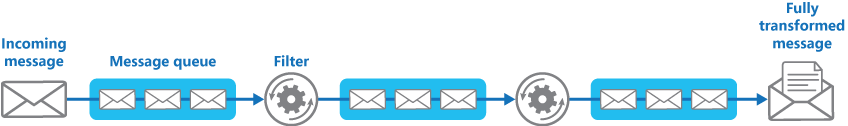
\includegraphics[scale=0.5]{pipes_and_filters_microsoft.png}  
    \caption{Схема реализации шаблона <<Каналы и фильтры>> от Microsoft}
    \label{fig:creation:pipes_and_filters_microsoft}
\end{figure}

Описанная реализация фокусируется на возможности распределенных вычислений которая в контексте обработки изображений бесполезно, поскольку производительность полученная от распределения фильтров на различные машины будет нивелированна временем затраченным передачу обрабатываемого изображения по сети. Главная цель при при использовании шаблона <<Каналы и фильтры>> в данном программном средстве это улучшение качества кода с точки зрения читаемости и модифицируемости. Декомпозиция кода на отдельные фильтры обработчики помогает упростить тестирование и реализацию отдельных модулей а правильная реализация каналов поможет в понимании связи фильтров и того что в целом происходит при обработке изображения. 

Прежде чем приступить к рассмотрению иходного кода требуется определить вспомогательные классы. 
В листинге \ref{lst:creation:result} приведена чать описания класса Result.
\begin{lstlisting}[style=fsharpstyle, caption={Определение вспомогательного класса Result}, label=lst:creation:result]
public class Result
{
  protected Result(bool success, string error)
  {
    Success = success;
    Error = error;
  }
  public bool Success { get; private set; }
  public bool Failed => !Success;
  public string Error { get; private set; }
  
  // ... 
}
\end{lstlisting}
Данный класс предназначен для упрощения обработки ошибок: все методы которые могут завершится неудачей должны возвращать класс Result не создавая при этом исключительных ситуаций. Использование описанной техники вместо исключительных ситуаций делает код понятнее потому как он исполняется последовательно как этого требует структурное программирование \cite{structured_programming}. Так же в программном средстве используется техника помогающая бороться с ошибками связанными с null значением. Это очень большая проблема для программистов! Техника состоит из 2 частей, первая это библиотека NullGuard \cite{null_guard}, которая встраивается в процесс компиляции и в начало каждого метода добавляет код проверяющий все входящие параметра на null значения, и в конец метода код проверяющий выходящее значение на null. Это запретит разработчику использовать null значения. Но для тех ситуаций где действительно значение может быть а может и не быть введем класс Maybe, код которого представлен на листинге \ref{lst:creation:maybe}. Приведенный выше подход помогает четко разделить в коде значения которые могут принимать значения null а какие нет.
\begin{lstlisting}[style=fsharpstyle, caption={Определение вспомогательного класса Maybe}, label=lst:creation:maybe]
public struct Maybe<T>
{
  private readonly T _value;
  public T Value
  {
    get
    {
      if (HasNoValue)
      {
        throw new NotSupportedException("Maybe has not value");
      }
        return _value;
      }
    }
  }
  public bool HasValue => return _value != null; 
  public bool HasNoValue => !HasValue;
  private Maybe([AllowNull] T value)
  {
    _value = value;
  }
  public static implicit operator Maybe<T>([AllowNull] T value)
  {
    return new Maybe<T>(value);
  }
}
\end{lstlisting}

Рассмотрим реализацию архитектурного шаблона <<Каналы и фильтры>>. В листинге \ref{lst:creation:ifilter} можно увидет определение интерфейса для фильтра. 
\begin{lstlisting}[style=fsharpstyle, caption={Определение интерфейса для фильтра}, label=lst:creation:ifilter]
public interface IFilter<in TIn, TOut> 
{
	Result<TOut> Process(TIn input);
}
\end{lstlisting}
Интерфейс фильтр определяет сущность производящую определенную операцию над входящими данными и возвращающую результат либо ошибку. На изображении \ref{fig:creation:filters_uml} представленна UML диаграмма классов фильтров используемых в проекте.
\begin{figure}[ht] 
    \centering
    \includegraphics[width=\textwidth]{filters_uml.png}  
    \caption{UML диаграмма фильтров}
    \label{fig:creation:filters_uml}
\end{figure}

Перед рассмотрением каналов следует рассмотреть ещё один полезный при разработке прием это <<Dependency injection>> что означает на русском звучит как внедрение зависимостей, это процесс предоставления внешней зависимости программному модулю. Идея заключается в том что каждый модуль описывает свои зависимости, и выделяется отдельный модуль занимающийся предоставлением зависимостей. В \csharp{} хорошей практикой считается описывать зависимости именно в конструкторе класса. На внешний модуль занимающийся подстановкой возложенна задача управления жизненным циклом объектов а также их созданем, этот модуль называют <<IoC>>. В \dotnet{} существует масса реализаций, я же в своем проекте использую реализацию от Microsoft называемую Unity потому как при всей гибкости настроек и удобства использования, это реализация показал отличные результаты в плане производительности \cite{ioc_perfomance}.

И так при создании канала были следующие задачи:
\begin{itemize}
  \item обеспечение связи между фильтрами, т.е. передача данных между фильтрами;
  \item связи могут быть нелинейными;
  \item связи могу быть один ко многим и много к одному;
  \item при создании фильтров использовать технику <<Dependency injection>>;
  \item должна быть проверка совместимости типов фильтров на этапе компиляции;
\end{itemize}

Под нелинейными связями подразумевались связи при которых данные идут в обход некоторых фильтров попадая к следующим. Пример нелинейного соединения данных можно увидеть на рисунке \ref{fig:creation:unlinear_filter_connection}, тут данные из процесса 1 идет в обход процесса 2 и 3 к процессу 4.
\begin{figure}[ht] 
    \centering
    \includegraphics[width=0.95\textwidth]{unlinear_filter_connection.png}  
    \caption{Диаграмма потока данных при нелинейных связях фильтрах}
    \label{fig:creation:unlinear_filter_connection}
\end{figure}

На рисунке \ref{fig:creation:filters-one-to-many} изображен пример связи между фильтрами один ко многим, на диаграмме процесс 1 создает множество потоков данных, кажный из которых проходит другие процессы, затем процесс $n+1$ принимает множество потоков данных.
\begin{figure}[ht] 
    \centering
    \includegraphics[scale=0.6]{filters-one-to-many.png}  
    \caption{Диаграмма потока данных при связях фильтров один ко многим}
    \label{fig:creation:filters-one-to-many}
\end{figure}

Использование техники <<Dependency injection>> означает то, что каждый фильтр должен иметь возможность определить свои зависимости в конструкторе, при этом не вызывая ошибок компиляции после добавления новой зависимости.

Проверка совместимости типов фильтров на этапе компиляции означает то, что в случае совмещения выхода фильтра $A$ и входа фильтра $B$ код будет компилироваться только в том случае, если выходным значением фильтра $A$ будет тип $a$ а входным значением фильтра $B$ будет тип $b$ такие что $a \geq b$.

Для реализации микроядерной архитектуры мы будем использовать загрузку .net сборок. Для каждой 